\documentclass[letterpaper,12pt]{article}
\usepackage{opticameet3}
\newcommand\authormark[1]{\textsuperscript{#1}}

\graphicspath{ {./images/} }
\usepackage[font=footnotesize]{caption}
\usepackage{tabularx}

% \usepackage{floatrow} % Commented out to avoid conflicts with minipage
\usepackage{amsmath,amssymb}
\usepackage{multicol}

\usepackage{float}
\usepackage{listings}
\geometry{letterpaper}
\usepackage{xcolor}

\usepackage{setspace}


\bibliographystyle{unsrt}
\def\bibfont{\footnotesize}

\geometry{left=1in,right=1in,top=1in,bottom=2in}
\hbadness=99999
\tolerance=10000
\setlength{\headheight}{14.49998pt}

\usepackage{fancyhdr} % Include the fancyhdr package
\usepackage{lipsum}   % For dummy text

% Configure the fancyhdr package
\pagestyle{fancy}     % Activate the fancyhdr package

% Clear default header and footer styles
\fancyhf{}


% Set header contents
\fancyhead[L]{\textbf{Spring 2025}} % Left-aligned
\fancyhead[C]{\textbf{Honors Report}} % Left-aligned
\fancyhead[R]{\textbf{\thepage}}          % Right-aligned (Page number)


% Define colors for syntax highlighting
\definecolor{codegreen}{rgb}{0,0.6,0}
\definecolor{codegray}{rgb}{0.5,0.5,0.5}
\definecolor{codepurple}{rgb}{0.58,0,0.82}
\definecolor{backcolour}{rgb}{0.97,0.97,0.98}


% Configure Python listing style
\lstdefinestyle{python}{
    backgroundcolor=\color{backcolour},
    commentstyle=\color{codegreen},
    keywordstyle=\color{magenta},
    numberstyle=\tiny\color{codegray},
    stringstyle=\color{codepurple},
    basicstyle=\ttfamily,            % Use tiny font size
    breakatwhitespace=false,
    breaklines=true,
    captionpos=b,
    keepspaces=true,
    numbers=left,
    numbersep=5pt,
    showspaces=false,
    showstringspaces=false,
    showtabs=false,
    tabsize=4,
    frame=single,                    % Add frame around the code
    framesep=2pt,                    % Small frame separation
    framerule=0pt,                 % Thin frame rule
    xleftmargin=10pt,
    xrightmargin=10pt,
    % Python specific settings
    language=Bash,
    morekeywords={self},             % Add self as a keyword
    emph={MyClass,__init__},         % Add custom highlighting for classes
    emphstyle=\color{blue},
}


\date{\today}

\usepackage{xcolor}
\definecolor{violet}{HTML}{3300AD}
\usepackage[colorlinks=true,bookmarks=false,citecolor=blue,urlcolor=blue,linkcolor=violet]{hyperref}
\begin{document}
\begin{spacing}{1.125}

    \title{\Large{Honors Report} \\ \normalsize{Spring 2025} \\ \vspace{1cm} \Huge{Study of Machine Learning models in the field of Particle Physics.
}}
\begin{figure}[H]
    \centering

\includegraphics[width=0.5\textwidth]{iiith_logo.png}
\end{figure}
\vspace{0.5cm}

\vspace{1cm}
\author{Abhiram Tilak - 2022113011}
\address{\authormark{*}International Instituite of Information Technology, Hyderabad}
\vspace{1cm}

\begin{abstract}
This report goes over a detailed classification of the different types of machine learning models used in the field of particle physics. 

Note that the purpose of this study is not to perform a deep dive on the architectural specifcations of each model, most of the discussion focuses on the applications of the models in the field of particle physics. We preset a brief overview of the different types of models used in the field of particle physics.
\end{abstract}

\pagebreak





\tableofcontents
\listoffigures
\listoftables
\lstlistoflistings


\section{Introduction}


ML methods are designed to harness large amounts of data in order to infer new information, making them naturally suited to various data processing tasks in Particle Physics,
from the moment a particle hits the detector all the way to the final published results.
The examples that follow give a representative idea of how extensively this technology has pervaded
the experiment, but merely scratch the surface of the full picture and potential of ML in HEP.

The application of machine learning techniques is gaining momentum in the research field of high energy physics (HEP) and astroparticle physics.
The experiments at large hadron collider (LHC) as well as several other collider-based and astroparticle experiments are accumulating large
amounts of data for the precision measurement of parameters of the Standard Model of particle physics and to search for existence of beyond
Standard Model physics at higher energy scale for which there are compelling theoretical and experimental reasons.

In the future, the high luminosity LHC is expected to deliver ten times more data than what is available till date.
Already, remarkable progress has been achieved in the application of machine learning in HEP,
in terms of developing event classification, object identification, and estimation strategies.
ML methods are expected to be heavily employed in future data analysis.\cite{atlas_ml}

\subsection{Types of Tasks in Particle Physics}

Before diving into different ML models, it is important to understand the types of tasks that are performed in particle physics
to understand why machine learning was even considered in the first place.

We can divide these tasks into two broad categories:
\begin{itemize}
  \item \textbf{Classification}: Categorizing events or particles into predefined classes.
  \begin{itemize}
      \item \textit{Jet Tagging}: Classifying jets (collimated sprays of particles) based on the type of fundamental particle (e.g., quark, gluon, or heavy quarks like $b$ or top quarks) that produced them. This is crucial for identifying decay products and understanding underlying physical processes.
      \item \textit{Particle Identification}: Distinguishing between particle types (e.g., electrons, muons, protons, pions) using their detector signatures. This is essential for accurate event reconstruction.
      \item \textit{Signal vs. Background Discrimination}: Detecting rare signal events amidst a larger background. This is often framed as a binary classification problem.
      \item \textit{Event Filtering (Trigger Systems)}: Real-time classification in detector trigger systems to decide which events to retain for analysis due to high collision rates.
  \end{itemize}

  \item \textbf{Regression}: Predicting continuous values from data.
  \begin{itemize}
      \item \textit{Energy and Momentum Regression}: Estimating particle or jet energy and momentum from detector signals, which often exhibit complex, non-linear responses.
      \item \textit{Vertex Position Estimation}: Determining the spatial origin of particle interactions within the detector.
      \item \textit{Tracking}: Reconstructing trajectories of charged particles. While tracking involves pattern recognition, refining trajectory parameters is treated as a regression task.
  \end{itemize}
\end{itemize}

\begin{figure}[H]
\centering
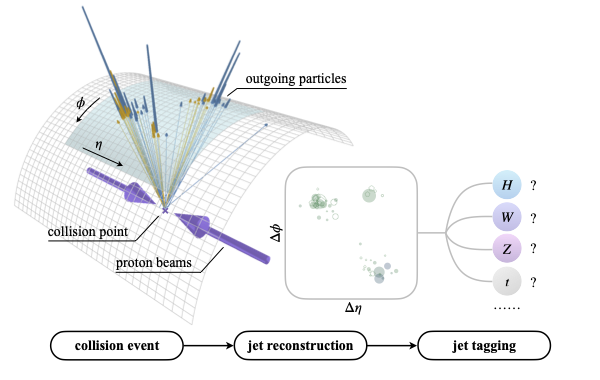
\includegraphics[width=0.7\textwidth]{jet-tagging.png}
\caption{ An example of jet tagging, where jets are classified based on the type of fundamental particle that produced them.}
\end{figure}

There are also methods don't fit neatly into these categories, such as:
\begin{itemize}
\item \textbf{Anomaly Detection}: Identifying events that deviate from expected patterns, potentially pointing to new physics beyond the Standard Model.

\item \textbf{Simulation}: Generating realistic synthetic data for analysis and comparison with theoretical models.

\item \textbf{Unfolding}: Correcting for detector effects to recover true distributions of physical quantities. Machine learning models are used to invert the detector response.
\end{itemize}
\vspace{1cm}
\begin{figure}[H]
\begin{minipage}{0.55\textwidth}
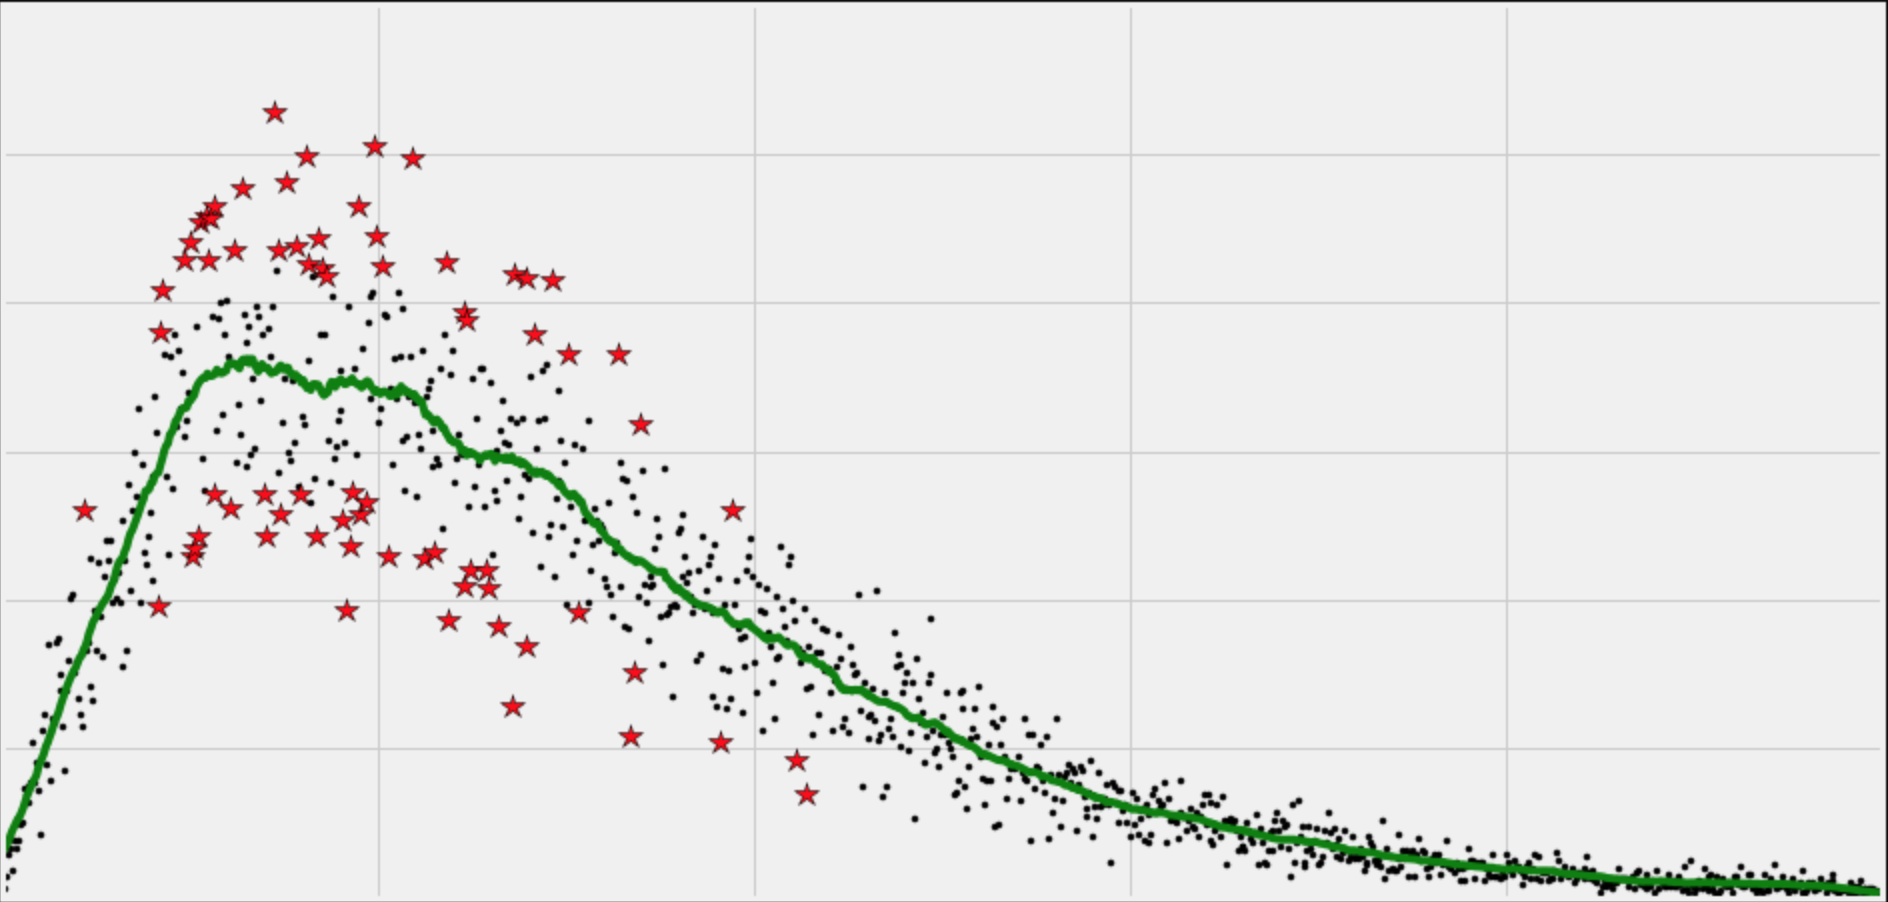
\includegraphics[width=\textwidth]{anomalies.png}
\end{minipage}
\hfill
\begin{minipage}{0.4\textwidth}
\caption{In ML for HEP, anomaly detection is used to identify events that deviate from expected patterns, potentially pointing to new physics beyond the Standard Model.}
\end{minipage}
\end{figure}

\section{Different types of models in HEP}


Based on the architecture used by the models, we can divide models into various categories.
\footnote{
\textbf{Note: } Each of these models can solve various different tasks in HEP, and the same task can be solved using different models. The choice of model depends on the specific problem, data characteristics, and computational resources available.
 For instance if we take an example from the NLP field can be adapted to solve a different task. For example, BERT, which is primarily used for text classification, can also be adapted for tasks like named entity recognition or question answering. Similarly, models like GPT-3, originally designed for text generation, can be fine-tuned for various NLP tasks such as summarization or translation.
}

\subsection{ Generative Models}

Generative models are particularly valuable in HEP for tasks involving the creation of realistic simulated data or modeling complex data distributions.

Generative models focus on learning underlying probability distributions to generate new, synthetic samples that resemble real data. These models are particularly valuable in HEP for simulation and data augmentation tasks.

\begin{figure}[H]
\centering
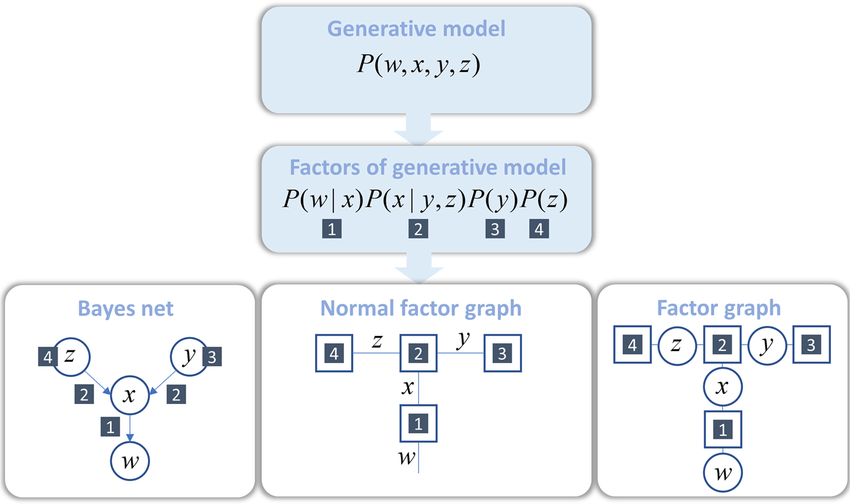
\includegraphics[width=0.9\textwidth]{generative.png}
\caption{A graphical representation of a probabilistic model.}
\end{figure}

\begin{itemize}
    \item \textbf{Fast Detector Simulation}: Traditional simulation methods like GEANT4\cite{geant4} are computationally expensive. Generative models such as GANs and VAEs are being developed to produce synthetic detector responses that are significantly faster while maintaining fidelity to real detector characteristics. This is essential for generating large simulated datasets, especially as LHC luminosity increases.
    
    \item \textbf{Event Generation}: Generative models are being explored to model and generate entire events or specific components, with the goal of accelerating parts of the simulation chain.
    
    \item \textbf{Modeling Complex Distributions}: These models can learn the probability distributions underlying high-dimensional collision data, aiding in understanding event structures and supporting tasks like anomaly detection.
    
    \item \textbf{Data Augmentation}: Creating synthetic but realistic variations of existing data to expand training datasets, particularly for rare processes.
\end{itemize}

Some popular examples of models in this category include:
    \subsubsection{CaloGAN\cite{calogan}}  
    CaloGAN represents a breakthrough application of Generative Adversarial Networks (GANs) for simulating electromagnetic showers in multi-layer calorimeters. Developed to address the computational bottleneck in traditional Monte Carlo simulation methods, CaloGAN can generate synthetic calorimeter responses with remarkable speed improvements.
    What differentiates CaloGAN from other generative approaches is its physics-aware architecture that preserves essential calorimeter shower properties while maintaining the enormous speed advantage. This model demonstrates how deep learning techniques can significantly accelerate one of the most computationally expensive steps in HEP simulation pipelines without sacrificing physical accuracy.

    \subsubsection{Variational Autoencoders} 
    Another important generative approach in HEP employs Variational Autoencoders (VAEs). A notable implementation described in a 2020 paper introduces a specialized VAE architecture for generating realistic and diverse jet images in high energy physics events
    The latent space characteristics of VAEs provide an interpretable representation that can be manipulated to generate specific physics scenarios, offering advantages for tasks like jet tagging evaluation and uncertainty quantification that may be more challenging with other generative approaches.

    \begin{figure}[H]
\centering
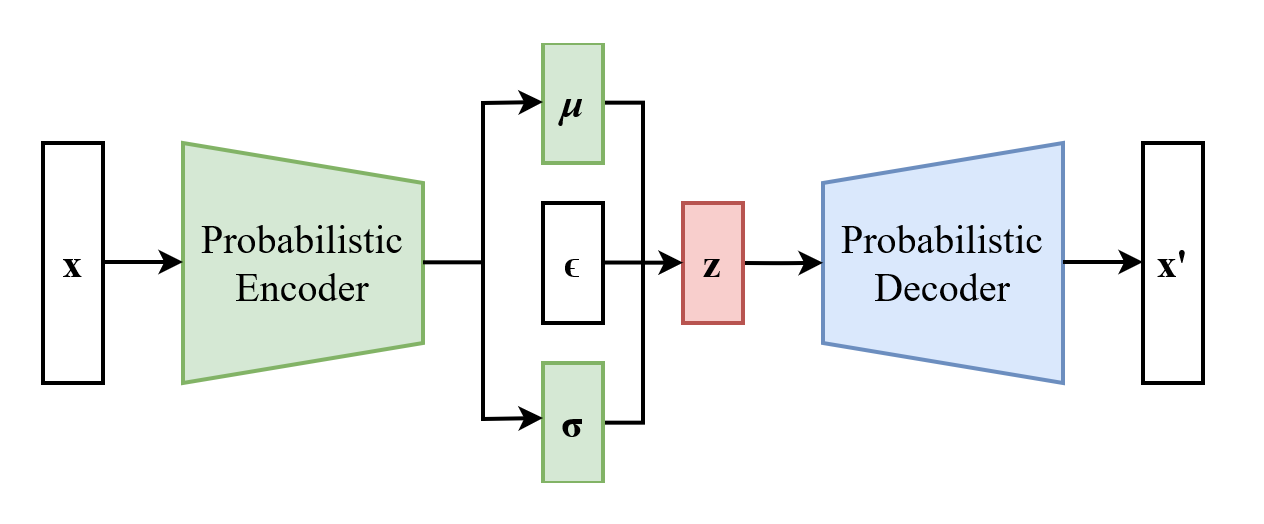
\includegraphics[width=0.7\textwidth]{variaitonal-autoencoders.png}
\caption{architecture of a variational autoencoder (VAE) for generating realistic and diverse jet images.}
    \end{figure}

\subsection{Discriminative Models}

Discriminative models are widely used for tasks where the goal is to differentiate between classes or predict values, typically under supervised learning.

Discriminative models excel at classification and regression tasks, learning boundaries between different classes of data-capabilities that are essential for many core HEP analysis requirements.

\begin{itemize}
    \item \textbf{Jet Tagging}: Classification of jets based on particle content and energy distribution to determine origin (e.g., $b$-jet, top-jet, quark-jet, gluon-jet), using models like deep neural networks, BDTs, and SVMs.
    
    \item \textbf{Particle Identification (PID)}: Classifying tracks or energy deposits to identify particles such as electrons, muons, photons, and protons—critical for event reconstruction.
    
    \item \textbf{Signal vs. Background Classification}: Classifying events to separate Standard Model backgrounds from potential new physics signals—a core task in discovery physics.
    
    \item \textbf{Event Filtering (Triggers)}: Discriminative models are used in trigger systems to make real-time decisions about which events to keep for offline analysis.
    
    \item \textbf{Regression for Physics Object Properties}: Predicting properties such as jet energy or vertex positions from raw detector data using regression models.
\end{itemize}

\subsubsection{ParticleNet\cite{particlenet}}

ParticleNet represents a state-of-the-art discriminative model specifically designed for jet tagging tasks in particle physics. The model employs a graph neural network architecture that treats jets as "particle clouds"-collections of individual particles with their associated properties.



\begin{figure}[H]
    \centering
    \begin{minipage}{0.48\textwidth}
        \centering
        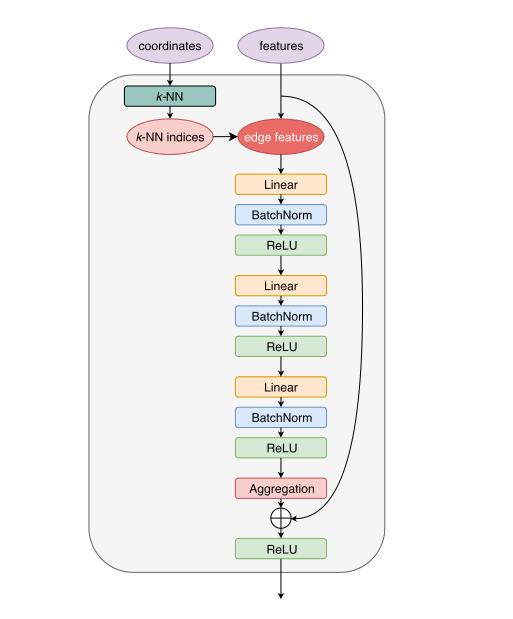
\includegraphics[width=\textwidth]{edge_conv.png}
        \caption[Architecture of ParticleNet]{The EdgeConv block in ParticleNet operates on particle clouds by dynamically building a graph for each particle based on its k-nearest neighbors. It computes edge features representing the relationship between a particle and its neighbors, which are then processed by a shared MLP. An aggregation step combines these features to create an enriched feature vector for each particle, allowing the network to learn local structures in the particle cloud in a permutation-invariant manner.}
    \end{minipage}
    \hfill
    \begin{minipage}{0.48\textwidth}
        \centering
        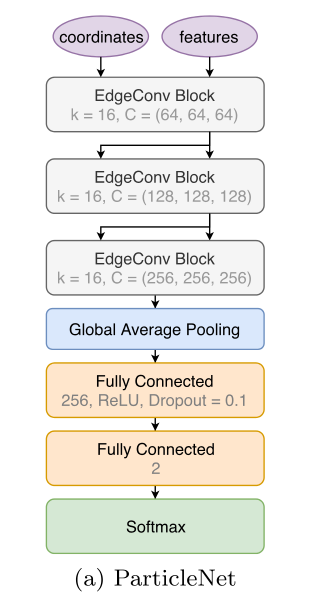
\includegraphics[width=0.8\textwidth]{particleNet.png}
        \caption[architecture of EdgeConv block in ParticleNet]{The architecture of the ParticleNet network. The ParticleNet architecture consists of three EdgeConv blocks. After the EdgeConv blocks, a channel-wise global average pooling operation is applied to aggregate the learned features over all particles in the cloud. This is followed by a fully connected layer with 256 units and the ReLU activation, and a dropout layer. A fully connected layer with two units, followed by a softmax function, is used to generate the output for the binary classification task.}
    \end{minipage}
\end{figure}

What sets ParticleNet apart from alternative approaches is its significantly improved performance combined with computational efficiency. When compared to image-based deep neural networks like ResNeXt-50 or other particle-based networks like P-CNN and PFN, ParticleNet achieves superior performance on both top tagging and quark-gluon tagging benchmarks. Remarkably, it accomplishes this with substantially fewer parameters-4 times fewer than ResNeXt-50 for the standard version and 56 times fewer for the lightweight version. This efficiency makes ParticleNet particularly valuable for applications with stringent latency and memory constraints, such as online event processing in HEP experiments.

\subsection{ Unsupervised Learning Models}

Unsupervised learning is applied when labels are not available, with the goal of discovering patterns or anomalies.

Unsupervised learning models discover patterns in data without labeled examples, making them valuable for anomaly detection and dimensionality reduction in HEP contexts.

\begin{itemize}
    \item \textbf{Anomaly Detection}: Detecting events that deviate from expected Standard Model patterns, potentially signaling new physics. Techniques include autoencoders (which detect anomalies via reconstruction error) and clustering approaches.
    
    \item \textbf{Clustering}: Grouping similar data points (e.g., calorimeter deposits or tracks). ML-based clustering can enhance or replace traditional algorithms in tasks such as vertex or shower reconstruction.
    
    \item \textbf{Dimensionality Reduction}: Reducing input feature space for visualization or preprocessing using techniques like PCA and t-SNE, while retaining essential data characteristics.
\end{itemize}

\subsection{Reinforcement\cite{Reinforcement} Learning in HEP}

Although less commonly used for direct data analysis, reinforcement learning is increasingly applied to system optimization.

\begin{itemize}
    \item \textbf{Particle Accelerator Control}: Tuning accelerator parameters to optimize performance metrics like beam intensity and stability via interaction with control systems.
    
    \item \textbf{Detector Operation Optimization}: Potential use in real-time detector configuration to enhance data acquisition and quality.
    
    \item \textbf{Event Reconstruction Algorithms}: Exploring sequential decision-making with reinforcement learning in reconstruction tasks, such as deciding how to associate detector hits into tracks.
\end{itemize}


\newcolumntype{L}[1]{>{\raggedright\arraybackslash}p{#1}} % custom left-aligned column
\begin{table}[H]
    \centering
    \caption{Classification of selected machine learning and deep learning models in HEP by learning paradigm.}
    \renewcommand{\arraystretch}{1.2}
    \begin{tabularx}{\textwidth}{|L{3cm}|L{2.5cm}|X|X|}
    \hline
    \textbf{Model Name} & \textbf{Category} & \textbf{Primary Application(s)} & \textbf{Notable Features / Comments} \\
    \hline
    CaloGAN\cite{calogan} & Generative & Calorimeter simulation (3D EM showers) & GAN-based generative model for fast simulation of electromagnetic showers\footnote{contentReference[oaicite:0]{index=0}}. \\
    \hline
    Normalizing Flow (NF) & Generative & End-to-end event simulation & Flow-based invertible generative model with exact likelihood; used for full-chain event generation\footnote{contentReference[oaicite:1]{index=1}}. \\
    \hline
    Variational Autoencoder (VAE) & Unsupervised & Anomaly detection (new physics searches) & Latent-variable generative model for unsupervised anomaly detection in events\footnote{contentReference[oaicite:2]{index=2}}. \\
    \hline
    Autoencoder (AE) & Unsupervised & Anomaly detection (trigger filtering) & Compresses events and flags unusual events via high reconstruction error\footnote{contentReference[oaicite:3]{index=3}}. \\
    \hline
    Convolutional Neural Network (CNN) & Discriminative & Calorimeter imaging / trigger & Convolutional classifier for calorimeter data (pattern recognition); e.g. identifying displaced particle showers\footnote{contentReference[oaicite:4]{index=4}}. \\
    \hline
    DeepJet & Discriminative & Jet flavor tagging (b/c jets) & Deep neural network using full jet constituent information; improves heavy-flavor tagging performance\footnote{contentReference[oaicite:5]{index=5}}. \\
    \hline
    ParticleNet\cite{particlenet} & Discriminative (Graph-based) & Jet tagging (quark/gluon, top) & Dynamic graph CNN on particle clouds; permutation-invariant jet classifier\footnote{contentReference[oaicite:6]{index=6}}. \\
    \hline
    LorentzNet\cite{LorentzNet} & Discriminative (Graph-based) & Jet tagging & Lorentz-equivariant graph neural network for jets; uses Minkowski dot-product attention\footnote{contentReference[oaicite:7]{index=7}}. \\
    \hline
    GNN tracking pipeline\cite{gnntracking} & Graph-based (Supervised) & Charged particle track reconstruction & Graph neural network (message-passing) linking detector hits into tracks\footnote{contentReference[oaicite:8]{index=8}}. \\
    \hline
    \end{tabularx}
    \label{tab:mlhep_models}
\end{table}
\end{spacing}


\section{Conclusion}
These diverse machine learning approaches demonstrate how computational techniques are transforming high-energy physics research across multiple fronts. Generative models like CaloGAN and VAEs are dramatically accelerating simulation tasks. Discriminative models like ParticleNet are enhancing our ability to identify specific particle signatures. Unsupervised approaches including quantum autoencoders enable model-agnostic searches for new physics. Reinforcement learning techniques are optimizing the operation of experimental facilities themselves.

Each model type offers distinct advantages for specific HEP applications while sharing the common goal of expanding the capabilities of modern particle physics beyond what traditional analytical and computational methods can achieve. As both machine learning techniques and HEP research continue to advance, we can expect increasingly sophisticated integration of these approaches to address the field's most challenging problems.

\bibliography{cite}

\end{document}
